\documentclass[a4paper,12pt]{article} % добавить leqno в [] для нумерации слева
\usepackage[a4paper,top=1.3cm,bottom=2cm,left=1.5cm,right=1.5cm,marginparwidth=0.75cm]{geometry}
%%% Работа с русским языком
\usepackage{cmap}					% поиск в PDF
\usepackage{mathtext} 				% русские буквы в фомулах
\usepackage[T2A]{fontenc}			% кодировка
\usepackage[utf8]{inputenc}			% кодировка исходного текста
\usepackage[english,russian]{babel}	% локализация и переносы
\usepackage{multirow}

\usepackage{graphicx}

\usepackage{wrapfig}
\usepackage{tabularx}

\usepackage{hyperref}
\usepackage[rgb]{xcolor}
\hypersetup{
colorlinks=true,urlcolor=blue
}

%%% Дополнительная работа с математикой
\usepackage{amsmath,amsfonts,amssymb,amsthm,mathtools} % AMS
\usepackage{icomma} % "Умная" запятая: $0,2$ --- число, $0, 2$ --- перечисление

%% Номера формул
\mathtoolsset{showonlyrefs=true} % Показывать номера только у тех формул, на которые есть \eqref{} в тексте.

%% Шрифты
\usepackage{euscript}	 % Шрифт Евклид
\usepackage{mathrsfs} % Красивый матшрифт

%% Свои команды
\DeclareMathOperator{\sgn}{\mathop{sgn}}

%% Перенос знаков в формулах (по Львовскому)
\newcommand*{\hm}[1]{#1\nobreak\discretionary{}
{\hbox{$\mathsurround=0pt #1$}}{}}

%% Графики
\usepackage{tikz}
\usepackage{pgfplots}
\pgfplotsset{compat=1.9}

\date{\today}

\begin{document}

\begin{titlepage}
	\begin{center}
		{\large МОСКОВСКИЙ ФИЗИКО-ТЕХНИЧЕСКИЙ ИНСТИТУТ (НАЦИОНАЛЬНЫЙ ИССЛЕДОВАТЕЛЬСКИЙ УНИВЕРСИТЕТ)}
	\end{center}
	\begin{center}
		{\large Физтех-школа аэрокосмических технологий}
	\end{center}
	
	
	\vspace{4.5cm}
	{\huge
		\begin{center}
			{\bf Отчёт о выполнении лабораторной работы 1.2.1}\\
			Определение скорости полёта пули при помощи баллистического маятника
		\end{center}
	}
	\vspace{1cm}
	\begin{center}
		{\large Соболевский Фёдор Александрович \\
			\vspace{0.2cm}
			Б03-109}
	\end{center}
	\vspace{8cm}
	\begin{center}
		Октябрь 2021
	\end{center}
\end{titlepage}

\section{Аннотация}

В данной работе измерена скорость пуль, вылетающих из духового ружья, при помощи двух баллистических маятников разных типов. В ходе измерений и вычислений исследованы погрешности прямых и косвенных измерений, а также изучены отклонения значений скорости от средних с целью определить факторы, влияющие на скорость пуль.

\section{Теоретические сведения}

\subsection{Метод баллистического маятника, совершающего поступательное движение}

\begin{figure}[h]
\begin{center}
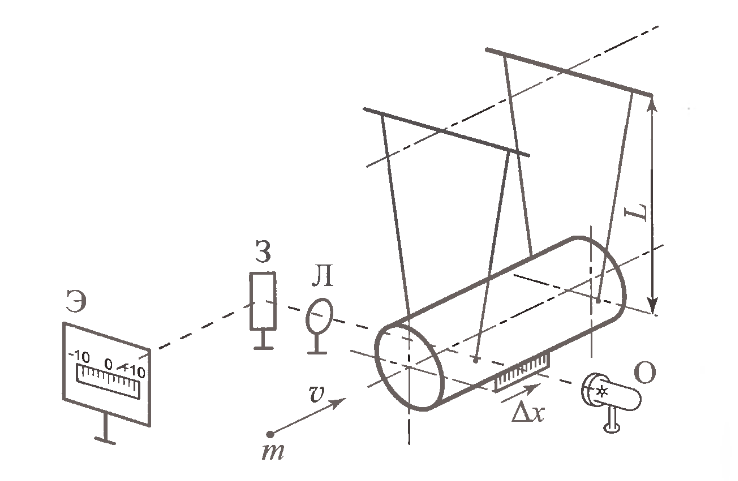
\includegraphics[width=0.6\textwidth]{prop-1.png}
\end{center}
\label{prop1}
\caption{Схема установки для измерения скорости полёта пули}
\end{figure}

\begin{figure}[h]
\begin{center}
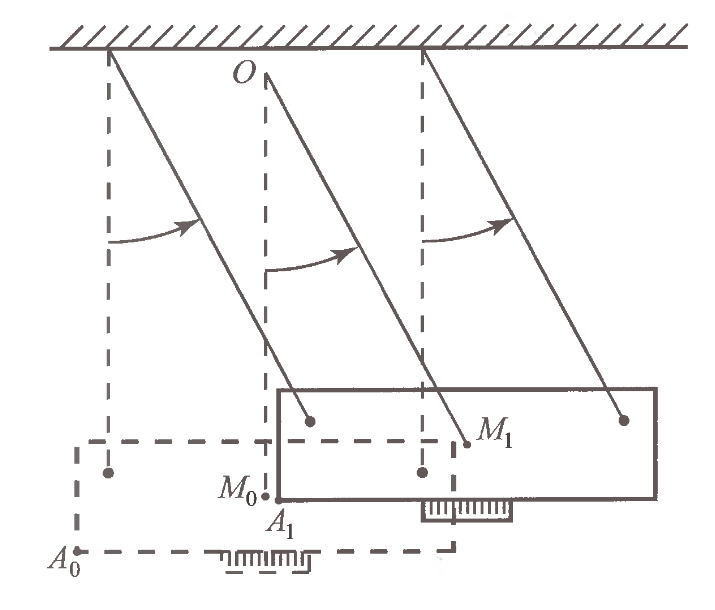
\includegraphics[width=0.6\textwidth]{prop-2.png}
\end{center}
\label{prop2}
\caption{Поступательное движение баллистического маятника при попадании в него пули}
\end{figure}

В первом опыте использовалась установка, изображенная на рисунке 1. Пусть масса маятника равна $M$, пули - $m$, причём $ m << M $. Тогда из закона сохранения импульса и скорости системы $ V $ сразу после столкновения можно найти скорость пули $ u $

\begin{equation}
mu = (M + m)V \text{,  } u = \frac{M + m}{m}V \approx \frac{M}{m}V
\label{impulse}
\end{equation}

При попадании пули маятник приобретает некоторую кинетическую энергию, которая при отклонении переходит в потенциальную. Пренебрегая потерями энергии, запишем закон сохранения механической энергии для маятника, где $ h $ - максимальная высота подъёма маятника, $ L $ - длина нитей подвеса:

\begin{equation}
    \frac{MV^2}{2}=Mgh \text{,    } V^2=2gh
    \label{energy}
\end{equation}

Высота подъёма маятника определяется через угол $ \varphi $ его отклонения от вертикали и величину $ \Delta x $ сдвига по горизонтальной оси как

\begin{equation}
    h = L(1 - \cos \varphi) = 2L \sin^2\frac{\varphi}{2} \text{,    где } \varphi \approx \frac{\Delta x}{L}
\end{equation}

Из \eqref{energy} и \eqref{impulse} скорость выражается, как

\begin{equation}
v = \sqrt{\frac{g}{L}}\frac{M}{m}\Delta x.
\end{equation}

\subsection{Метод крутильного баллистического маятника}

\begin{figure}[h]
\begin{center}
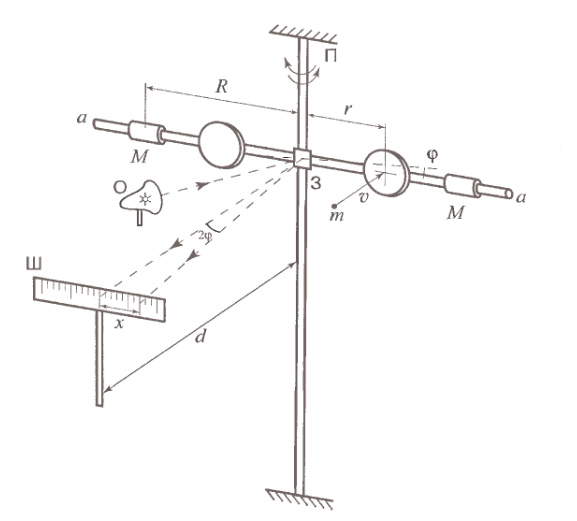
\includegraphics[width=0.73\textwidth]{rot.png}
\end{center}
\label{rot}
\caption{Схема установки для измерения скорости полёта пули с крутильным баллистическим маятником}
\end{figure}

Во втором опыте использовалась установка, изображенная на рисунке 3. Пуля массой $m$ попадает в мишень, закреплённую на стержне, которая вместе с дополнительным грузом массой M и проволокой П образует крутильный маятник. Считая удар пули абсолютно неупругим, для определения скорости $u$ пули можно воспользоваться законом сохранения момента импульса

\begin{equation}
    mur=I\Omega
    \label{inertia}
\end{equation}
где $I$ -- момент инерции системы маятника, $ \Omega $ - его угловая скорость сразу после удара.

Если $k$ -- модуль кручения проволоки, то из закона сохранения энергии следует, что

\begin{equation}
k \frac{\varphi^2}{2} = I \frac{\Omega^2}{2},
\label{turn}
\end{equation}

где $\varphi$ -- максимальный угол поворота маятника.

Из уравнений \eqref{inertia} и \eqref{turn} можно выразить скорость $u$

\begin{equation}
u = \varphi \frac{\sqrt{kI}}{mr}.
\label{velocity2}
\end{equation}

Угол $ \varphi $ в данном опыте вычислялся из величины $ x $ смещения изображения нити осветителя на измерительной шкале и расстояния $d$ от шкалы до оси вращения маятника

\begin{equation}
    \varphi \approx \frac{x}{2d}
\end{equation}

Величину $ \sqrt{kI} $ из формулы \eqref{velocity2} можно определить из периодов колебаний маятника с грузами M и без них. В первом случае период колебаний маятника равен

\begin{equation}
    T_1=2\pi\sqrt{\frac{I}{k}},
    \label{period1}
\end{equation}
во втором случае

\begin{equation}
    T_2=2\pi\sqrt{\frac{I - 2MR^2}{k}}
    \label{period2}
\end{equation}
где $ R $ - расстояние от центров масс грузов до проволоки.

Из \eqref{period1} и \eqref{period2} следует

\begin{equation}
    \sqrt{kI}=\frac{4\pi MR^2T_1}{T_{1}^2-T_{2}^2},
\end{equation}

\section{Оборудование и инстументальные погрешности}
\textbf{Оборудование:} духовое ружьё на штативе, осветитель, оптическая система для измерения отклонений маятника, баллистические маятники, пули.\\
\textbf{Измерительные приборы:}
\begin{itemize}
    \item \textbf{Весы: } $ \Delta_\text{вес} = 0,005$ г;
    \item \textbf{Линейка: } $ \Delta_\text{лин} = 1$ мм;
    \item \textbf{Измерительная шкала установки 1: } $ \Delta_\text{шк1} = 0,5$ мм;
    \item \textbf{Измерительная шкала установки 2: } $ \Delta_\text{шк2} = 1$ мм;
    \item \textbf{Секундомер: } $ \Delta_\text{сек} = 0.1$ с.
\end{itemize}

\section{Результаты измерений и обработка экспериментальных данных}

\subsection{Измерение масс и длин}

Массы пуль представлены в таблице \ref{mass}:

\begin{table}[h]
\begin{center}$
\begin{array}{|c|c|c|c|c|c|c|c|c|}
\hline
\text{№ пули} & 1 & 2 & 3 & 4 & 5 & 6 & 7 & 8  \\
\hline
m\text{, г} & 0.500 & 0.514 & 0.500 & 0.518 & 0.500 & 0.505 & 0.503 & 0.499  \\
\hline
\end{array}$
\end{center}
\label{mass}
\caption{Массы пуль}
\end{table}

Измерены величины $L = (2200\pm1)$ мм, $M=(2925\pm5)$ г для первого опыта и величины $ R = 335 \pm 1$ мм, $ r = 220 \pm 1$ мм, $ d = 500 \pm 1$ мм, $M = 729,5 \pm 5$ г.

Предварительное изучение установок показало, что затухание колебаний

\subsection{Результаты опыта с установкой 1}

Величины смещения $ \Delta x $, соответствующие скорости пулей и их отклонения от среднего значения представлены в таблице \ref{res1}: 

\begin{table}[h]
\begin{center}$
\begin{array}{|c|c|c|}
\hline
\Delta x\text{, мм} & u\text{, м/c} & u - \overline{u} \text{, м/с} \\
\hline
9,0 & 112,25 & 1,37\\
\hline
9,5 & 115,26 & 1,67\\
\hline
9,5 & 118,49 & 4,90\\
\hline
9,0 & 108,35 & 5,24\\
\hline
\end{array}$
\end{center}
\label{res1}
\caption{Результаты измерения скорости пуль в первом опыте}
\end{table}

Среднее значение $ \overline{u} = 113,6\text{ м/c}$. Систематическая погрешность определения скорости

\begin{equation}
    \sigma_{u1} = u\sqrt{(\frac{\Delta_\text{вес}}{M})^2 + (\frac{\Delta_\text{вес}}{m})^2 + \frac{1}{4}(\frac{\Delta_\text{лин}}{l})^2 + (\frac{\Delta_\text{шк1}}{\Delta x})^2} \approx 6,4 \text{ м/с}
\end{equation}

Итоговый результат:

\begin{itemize}
\item $ \overline{u_1} = 113,6 \pm 6,4 $ м/с
\end{itemize}

\subsection{Результаты опыта с установкой 2}

Периоды колебаний без грузов и с грузами составили $ T_1 = 15,3$ c и $ T_2 = 17,4$ c. Отсюда найдено значение

\begin{equation*}
\sqrt{\textit{kI}} = \frac{4 \pi M R^2 T_1}{T_1^2 - T_2^2} = 64,8\cdot 10^{-2} \: \text{кг} \cdot \text{м}^2 / \text{с}
\end{equation*}

Отсюда найдены значения скоростей, представленные в таблице \ref{tab3}, по формуле

\begin{equation}
v = \varphi \frac{\sqrt{kI}}{mr} = \frac{x}{2d}\frac{\sqrt{kI}}{mr}
\end{equation}

\begin{table}[h]
\begin{center}$
\begin{array}{|c|c|c|}
\hline
x\text{, мм} & u\text{, м/c} & u - \overline{u} \text{, м/с} \\
\hline
18,5 & 108,97 & 2,53\\
\hline
20,5 & 119,56 & 8,05\\
\hline
19,0 & 111,25 & 0,25\\
\hline
18,0 & 106,24 & 5,27\\
\hline
\end{array}$
\end{center}
\label{tab3}
\caption{Результаты измерения скорости пуль во втором опыте}
\end{table}

Систематическая погрешность вычисления скорости найдена по формуле

\begin{equation}
    \sigma_{u1} = u\sqrt{(\frac{\Delta_\text{вес}}{m})^2 + (\frac{\Delta_\text{лин}}{r})^2 + (\frac{\Delta_\text{лин}}{d})^2 + (\frac{\Delta_{\sqrt{kI}}}{\sqrt{kl}})^2 + (\frac{\Delta_\text{шк2}}{x})^2} \approx 8,9 \text{ м/с}
\end{equation}

Итоговый результат:

\begin{itemize}
\item $ \overline{u_2} = 111,5 \pm 8,9 $ м/с
\end{itemize}

\section {Обсуждение результатов и вывод}

В ходе данной работы получены значения скорости пуль с точностью до 5-8 \%, причём погрешеность измерений при использовании второй установки оказалась заметно больше из-за большего объёма вычислений. Полученной точности достаточно, чтобы убедиться в применимости использованных методов измерения скоростей. Однако наблюдается существенный разброс скоростей (около 10 м/с), причём между скоростями пуль и их массами невозможно установить однозначное соответствие. Это говорит о том, что на скорость пуль влияют внешние факторы, как то: сопротивление воздуха, начальное положение в духовом ружье и т.п.  

\end{document}